\documentclass[border=10pt]{standalone}

\usepackage{tikz}
\usepackage{tikzsymbols}
\usetikzlibrary{calc,patterns,shapes.geometric}

\def\centerarc[#1](#2)(#3:#4:#5){\draw[#1] ($(#2)+({#5*cos(#3)},{#5*sin(#3)})$) arc (#3:#4:#5);}

\begin{document}
	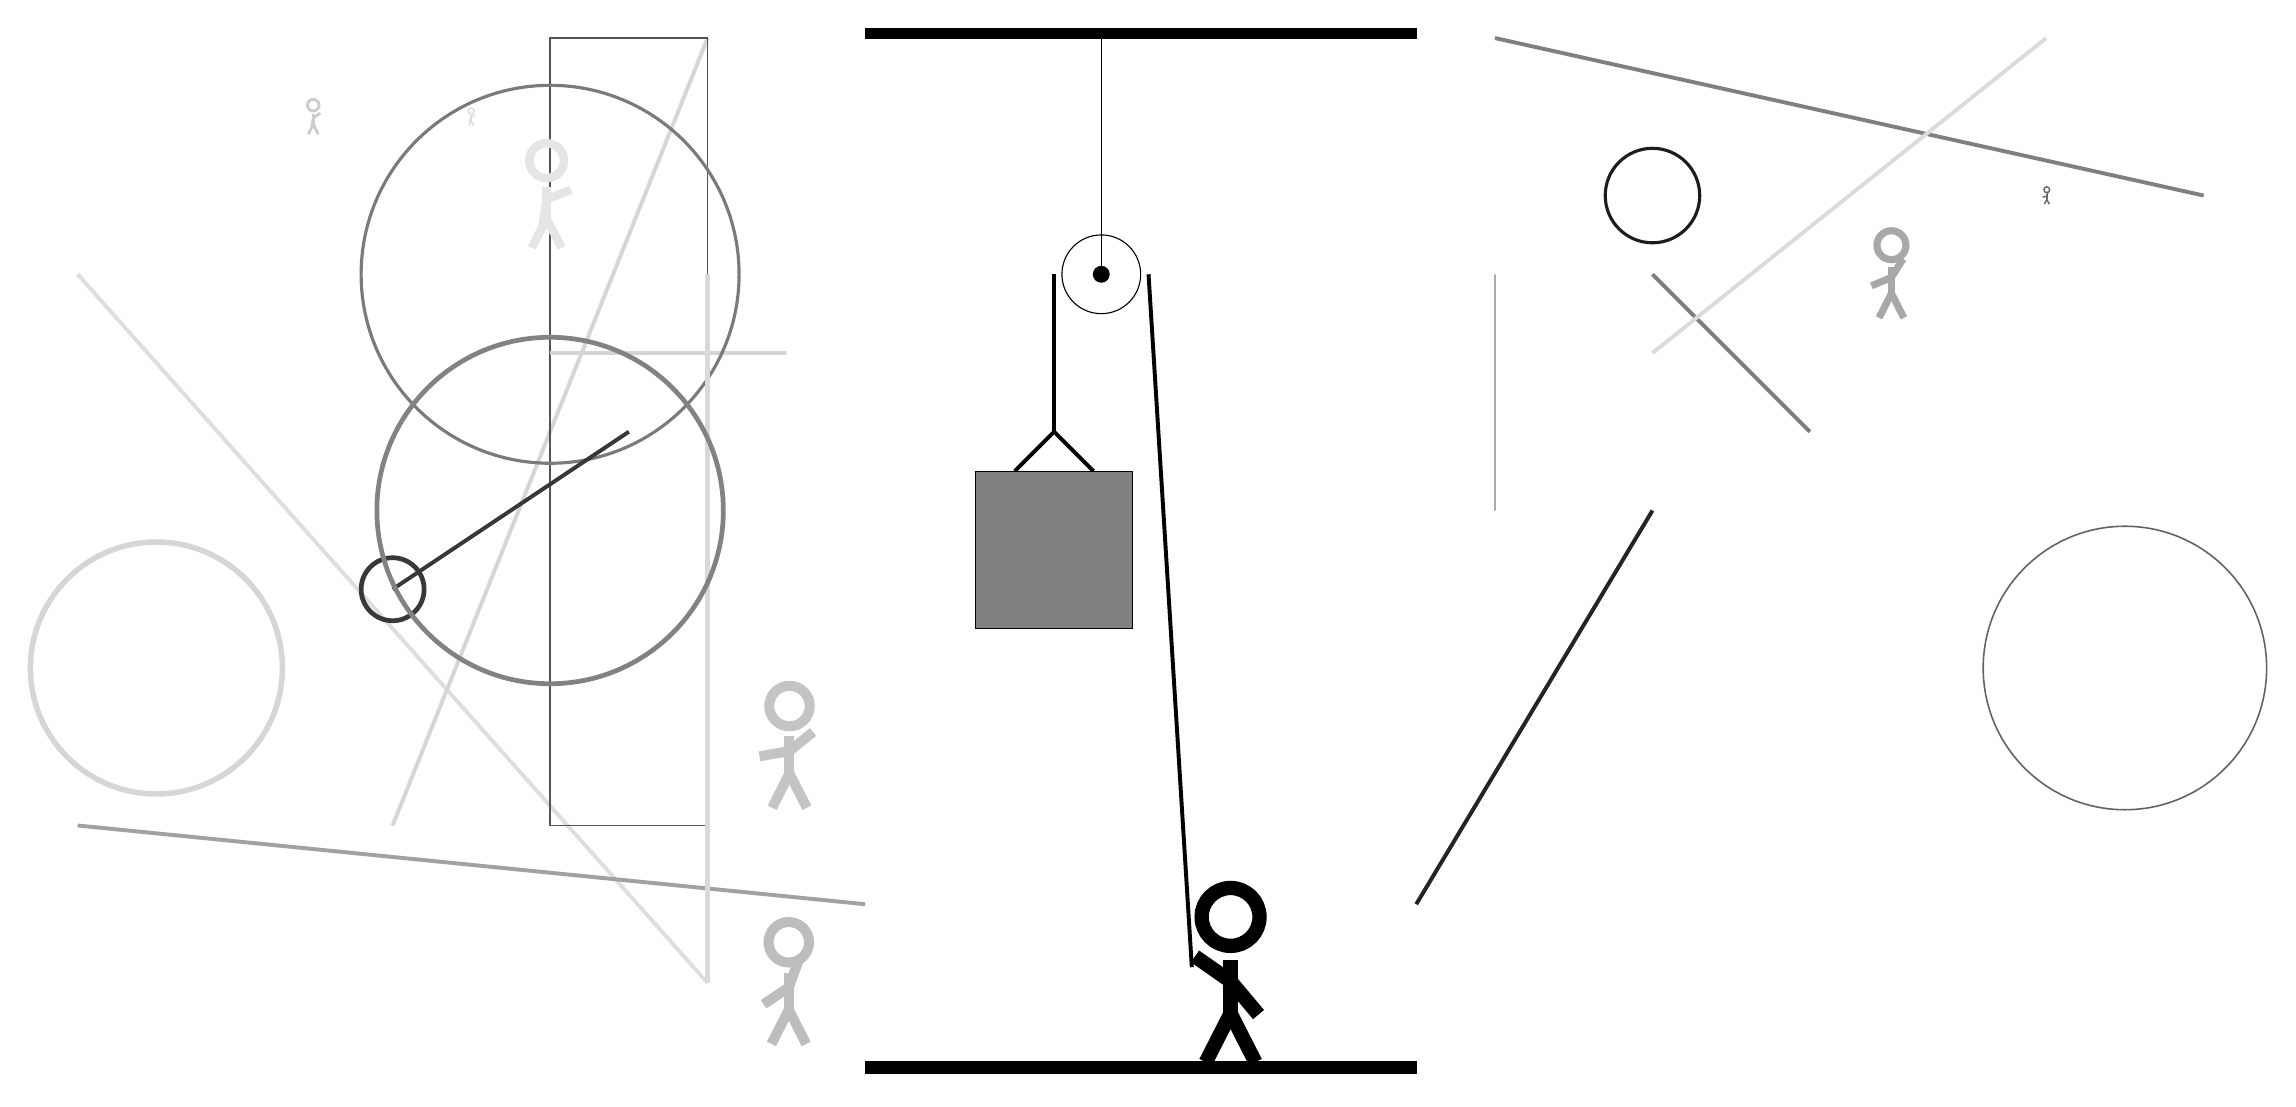
\begin{tikzpicture}
		%%%%% START %%%%%
		
		\draw[fill=black] (-2, 10) rectangle (5, 10.125);
		
		\draw [line width=0.4mm, color=black!89](8, 8) circle (0.6);
		
		\draw[line width=0.5mm, color=black!13](-4, -2) -- (-12, 7);
		\draw[line width=0.5mm, color=black!16](-4, 10) -- (-8, 0);
		\draw[line width=0.5mm, color=black!86](8, 4) -- (5, -1);
		
		\draw[line width=0.2mm, color=black!33] (6, 7) rectangle (6, 4);
		\draw[line width=0.2mm, color=black!67] (-4, 0) rectangle (-6, 10);
		\draw[line width=0.5mm, color=black!17] (-3, 6) rectangle (-6, 6);
		
		\draw [line width=0.6mm, color=black!78](-8, 3) circle (0.4);
		\draw [line width=0.4mm, color=black!52](-6, 7) circle (2.4);
		\draw[line width=0.5mm, color=black!51](8, 7) -- (10, 5);
		\node[line width=0.2mm, color=black!34] at (11, 7) {\Strichmaxerl[5][23][58]};
		\node[line width=0.2mm, color=black!59] at (13, 8) {\Strichmaxerl[1][15][75]};
		\draw [line width=0.2mm, color=black!62](14, 2) circle (1.8);
		
		\draw[line width=0.7mm, color=black!81] (-4, 1) rectangle (-4, 0);
		\draw[line width=0.5mm, color=black!50](6, 10) -- (15, 8);
		\draw [line width=0.7mm, color=black!16](-11, 2) circle (1.6);
		\draw[line width=0.7mm, color=black!66] (-4, -2) rectangle (-4, -2);
		
		\draw[line width=0.5mm, color=black!14](8, 6) -- (13, 10);
		\node[line width=0.6mm, color=black!10] at (-6, 8) {\Strichmaxerl[6][81][21]};
		\draw[line width=0.5mm, color=black!37](-2, -1) -- (-12, 0);
		\draw[line width=0.5mm, color=black!78](-5, 5) -- (-8, 3);
		
		\draw[line width=0.6mm, color=black!15] (-4, 7) rectangle (-4, -2);
		\draw [line width=0.6mm, color=black!49](-6, 4) circle (2.2);
		\node[line width=0.7mm, color=black!26] at (-3, -2) {\Strichmaxerl[7][34][70]};
		\node[line width=0.7mm, color=black!14] at (-7, 9) {\Strichmaxerl[1][59][41]};
		
		\node[line width=0.5mm, color=black!23] at (-3, 1) {\Strichmaxerl[7][10][39]};
		\node[line width=0.6mm, color=black!20] at (-9, 9) {\Strichmaxerl[2][80][36]};
		
		\draw (1, 7) circle (0.5);
		\draw[fill=black] (1, 7) circle (0.1);
		\draw (1, 10) -- (1, 7);
		
		\draw[line width=0.5mm] (-0.1, 4.5) -- (0.4, 5.0) -- (0.9, 4.5);
		\draw[fill=black!50] (-0.6, 4.5) rectangle (1.4, 2.5);
		
		\draw[line width=0.5mm] (0.4, 7) -- (0.4, 5.0);
		\centerarc[line width=0.5mm](1, 7)(0:180:0.6);
		\draw[line width=0.5mm](1.6, 7) -- (2.15, -1.8);
		
		\node at (2.6, -1.9) {\Strichmaxerl[10][-35][-50]};
		
		\draw[fill=black] (-2, -3) rectangle (5, -3.15);
		
		%%%%% END %%%%%
	\end{tikzpicture}
\end{document}